\documentclass{standalone}
\usepackage{tikz}
\usetikzlibrary{shapes,arrows.meta}

\begin{document}

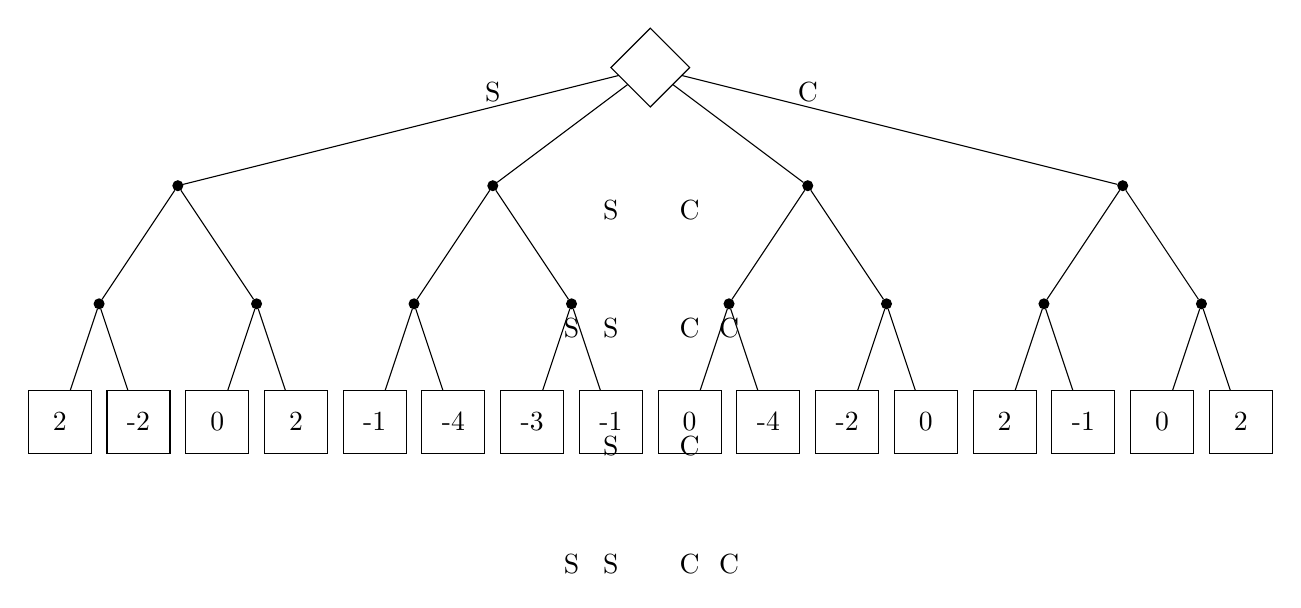
\begin{tikzpicture}[
  level distance=1.5cm,
  level 1/.style={sibling distance=4cm},
  level 2/.style={sibling distance=2cm},
  level 3/.style={sibling distance=1cm},
  every node/.style={inner sep=2pt, outer sep=0pt},
  decision/.style={diamond, draw, minimum size=1cm, inner sep=0pt},
  adversary/.style={circle, fill, minimum size=4pt, inner sep=0pt},
  payoff/.style={rectangle, draw, minimum size=0.8cm}
]

\node[decision] {} 
  child {node[adversary] {}
    child {node[adversary] {}
      child {node[payoff] {2}}
      child {node[payoff] {-2}}
    }
    child {node[adversary] {}
      child {node[payoff] {0}}
      child {node[payoff] {2}}
    }
  }
  child {node[adversary] {}
    child {node[adversary] {}
      child {node[payoff] {-1}}
      child {node[payoff] {-4}}
    }
    child {node[adversary] {}
      child {node[payoff] {-3}}
      child {node[payoff] {-1}}
    }
  }
  child {node[adversary] {}
    child {node[adversary] {}
      child {node[payoff] {0}}
      child {node[payoff] {-4}}
    }
    child {node[adversary] {}
      child {node[payoff] {-2}}
      child {node[payoff] {0}}
    }
  }
  child {node[adversary] {}
    child {node[adversary] {}
      child {node[payoff] {2}}
      child {node[payoff] {-1}}
    }
    child {node[adversary] {}
      child {node[payoff] {0}}
      child {node[payoff] {2}}
    }
  };

\foreach \i in {1,2,3,4} {
  \path (0,-1.5*\i) -- +(-0.5,-0.5) node[above] {S} -- +(0.5,-0.5) node[above] {C};
}

\foreach \i in {1,2} {
  \path (0,-3*\i) -- +(-1,-0.5) node[above] {S} -- +(1,-0.5) node[above] {C};
}

\path (0,0) -- +(-2,-0.5) node[above] {S} -- +(2,-0.5) node[above] {C};

\end{tikzpicture}

\end{document}